% Created by tikzDevice version 0.10.1 on 2018-02-02 18:17:28
% !TEX encoding = UTF-8 Unicode
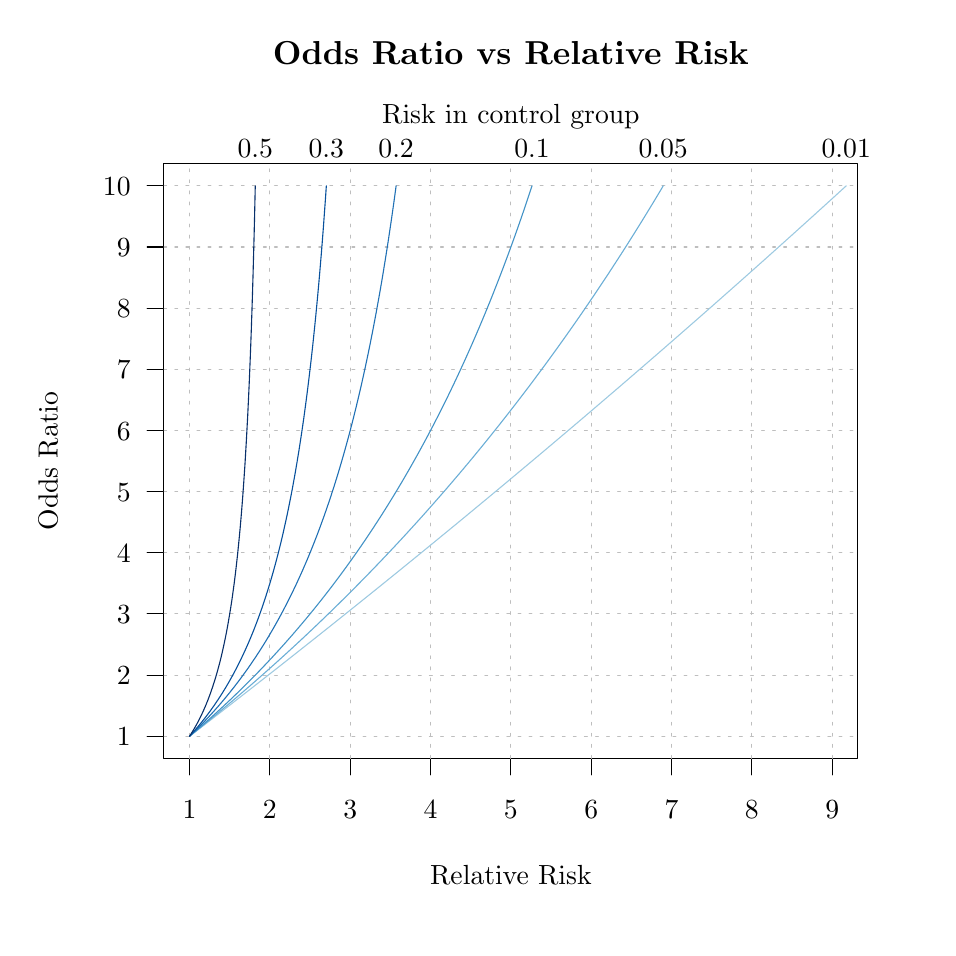
\begin{tikzpicture}[x=1pt,y=1pt]
\definecolor{fillColor}{RGB}{255,255,255}
\path[use as bounding box,fill=fillColor,fill opacity=0.00] (0,0) rectangle (325.21,325.21);
\begin{scope}
\path[clip] (  0.00,  0.00) rectangle (325.21,325.21);
\definecolor{drawColor}{RGB}{0,0,0}

\path[draw=drawColor,line width= 0.4pt,line join=round,line cap=round] ( 49.20, 61.20) --
	(300.01, 61.20) --
	(300.01,276.01) --
	( 49.20,276.01) --
	( 49.20, 61.20);
\end{scope}
\begin{scope}
\path[clip] (  0.00,  0.00) rectangle (325.21,325.21);
\definecolor{drawColor}{RGB}{0,0,0}

\node[text=drawColor,anchor=base,inner sep=0pt, outer sep=0pt, scale=  1.00] at (174.61, 15.60) {Relative Risk};

\node[text=drawColor,rotate= 90.00,anchor=base,inner sep=0pt, outer sep=0pt, scale=  1.00] at ( 10.80,168.61) {Odds Ratio};
\end{scope}
\begin{scope}
\path[clip] (  0.00,  0.00) rectangle (325.21,325.21);
\definecolor{drawColor}{RGB}{0,0,0}

\path[draw=drawColor,line width= 0.4pt,line join=round,line cap=round] ( 49.20, 69.16) -- ( 49.20,268.06);

\path[draw=drawColor,line width= 0.4pt,line join=round,line cap=round] ( 49.20, 69.16) -- ( 43.20, 69.16);

\path[draw=drawColor,line width= 0.4pt,line join=round,line cap=round] ( 49.20, 91.26) -- ( 43.20, 91.26);

\path[draw=drawColor,line width= 0.4pt,line join=round,line cap=round] ( 49.20,113.36) -- ( 43.20,113.36);

\path[draw=drawColor,line width= 0.4pt,line join=round,line cap=round] ( 49.20,135.46) -- ( 43.20,135.46);

\path[draw=drawColor,line width= 0.4pt,line join=round,line cap=round] ( 49.20,157.56) -- ( 43.20,157.56);

\path[draw=drawColor,line width= 0.4pt,line join=round,line cap=round] ( 49.20,179.66) -- ( 43.20,179.66);

\path[draw=drawColor,line width= 0.4pt,line join=round,line cap=round] ( 49.20,201.76) -- ( 43.20,201.76);

\path[draw=drawColor,line width= 0.4pt,line join=round,line cap=round] ( 49.20,223.86) -- ( 43.20,223.86);

\path[draw=drawColor,line width= 0.4pt,line join=round,line cap=round] ( 49.20,245.96) -- ( 43.20,245.96);

\path[draw=drawColor,line width= 0.4pt,line join=round,line cap=round] ( 49.20,268.06) -- ( 43.20,268.06);

\node[text=drawColor,anchor=base east,inner sep=0pt, outer sep=0pt, scale=  1.00] at ( 37.20, 65.71) {1};

\node[text=drawColor,anchor=base east,inner sep=0pt, outer sep=0pt, scale=  1.00] at ( 37.20, 87.81) {2};

\node[text=drawColor,anchor=base east,inner sep=0pt, outer sep=0pt, scale=  1.00] at ( 37.20,109.91) {3};

\node[text=drawColor,anchor=base east,inner sep=0pt, outer sep=0pt, scale=  1.00] at ( 37.20,132.01) {4};

\node[text=drawColor,anchor=base east,inner sep=0pt, outer sep=0pt, scale=  1.00] at ( 37.20,154.11) {5};

\node[text=drawColor,anchor=base east,inner sep=0pt, outer sep=0pt, scale=  1.00] at ( 37.20,176.21) {6};

\node[text=drawColor,anchor=base east,inner sep=0pt, outer sep=0pt, scale=  1.00] at ( 37.20,198.31) {7};

\node[text=drawColor,anchor=base east,inner sep=0pt, outer sep=0pt, scale=  1.00] at ( 37.20,220.41) {8};

\node[text=drawColor,anchor=base east,inner sep=0pt, outer sep=0pt, scale=  1.00] at ( 37.20,242.51) {9};

\node[text=drawColor,anchor=base east,inner sep=0pt, outer sep=0pt, scale=  1.00] at ( 37.20,264.62) {10};

\path[draw=drawColor,line width= 0.4pt,line join=round,line cap=round] ( 58.49, 61.20) -- (290.73, 61.20);

\path[draw=drawColor,line width= 0.4pt,line join=round,line cap=round] ( 58.49, 61.20) -- ( 58.49, 55.20);

\path[draw=drawColor,line width= 0.4pt,line join=round,line cap=round] ( 87.52, 61.20) -- ( 87.52, 55.20);

\path[draw=drawColor,line width= 0.4pt,line join=round,line cap=round] (116.55, 61.20) -- (116.55, 55.20);

\path[draw=drawColor,line width= 0.4pt,line join=round,line cap=round] (145.58, 61.20) -- (145.58, 55.20);

\path[draw=drawColor,line width= 0.4pt,line join=round,line cap=round] (174.61, 61.20) -- (174.61, 55.20);

\path[draw=drawColor,line width= 0.4pt,line join=round,line cap=round] (203.64, 61.20) -- (203.64, 55.20);

\path[draw=drawColor,line width= 0.4pt,line join=round,line cap=round] (232.67, 61.20) -- (232.67, 55.20);

\path[draw=drawColor,line width= 0.4pt,line join=round,line cap=round] (261.70, 61.20) -- (261.70, 55.20);

\path[draw=drawColor,line width= 0.4pt,line join=round,line cap=round] (290.73, 61.20) -- (290.73, 55.20);

\node[text=drawColor,anchor=base,inner sep=0pt, outer sep=0pt, scale=  1.00] at ( 58.49, 39.60) {1};

\node[text=drawColor,anchor=base,inner sep=0pt, outer sep=0pt, scale=  1.00] at ( 87.52, 39.60) {2};

\node[text=drawColor,anchor=base,inner sep=0pt, outer sep=0pt, scale=  1.00] at (116.55, 39.60) {3};

\node[text=drawColor,anchor=base,inner sep=0pt, outer sep=0pt, scale=  1.00] at (145.58, 39.60) {4};

\node[text=drawColor,anchor=base,inner sep=0pt, outer sep=0pt, scale=  1.00] at (174.61, 39.60) {5};

\node[text=drawColor,anchor=base,inner sep=0pt, outer sep=0pt, scale=  1.00] at (203.64, 39.60) {6};

\node[text=drawColor,anchor=base,inner sep=0pt, outer sep=0pt, scale=  1.00] at (232.67, 39.60) {7};

\node[text=drawColor,anchor=base,inner sep=0pt, outer sep=0pt, scale=  1.00] at (261.70, 39.60) {8};

\node[text=drawColor,anchor=base,inner sep=0pt, outer sep=0pt, scale=  1.00] at (290.73, 39.60) {9};
\end{scope}
\begin{scope}
\path[clip] ( 49.20, 61.20) rectangle (300.01,276.01);
\definecolor{drawColor}{RGB}{190,190,190}

\path[draw=drawColor,line width= 0.4pt,dash pattern=on 1pt off 3pt ,line join=round,line cap=round] ( 49.20, 69.16) -- (300.01, 69.16);

\path[draw=drawColor,line width= 0.4pt,dash pattern=on 1pt off 3pt ,line join=round,line cap=round] ( 49.20, 91.26) -- (300.01, 91.26);

\path[draw=drawColor,line width= 0.4pt,dash pattern=on 1pt off 3pt ,line join=round,line cap=round] ( 49.20,113.36) -- (300.01,113.36);

\path[draw=drawColor,line width= 0.4pt,dash pattern=on 1pt off 3pt ,line join=round,line cap=round] ( 49.20,135.46) -- (300.01,135.46);

\path[draw=drawColor,line width= 0.4pt,dash pattern=on 1pt off 3pt ,line join=round,line cap=round] ( 49.20,157.56) -- (300.01,157.56);

\path[draw=drawColor,line width= 0.4pt,dash pattern=on 1pt off 3pt ,line join=round,line cap=round] ( 49.20,179.66) -- (300.01,179.66);

\path[draw=drawColor,line width= 0.4pt,dash pattern=on 1pt off 3pt ,line join=round,line cap=round] ( 49.20,201.76) -- (300.01,201.76);

\path[draw=drawColor,line width= 0.4pt,dash pattern=on 1pt off 3pt ,line join=round,line cap=round] ( 49.20,223.86) -- (300.01,223.86);

\path[draw=drawColor,line width= 0.4pt,dash pattern=on 1pt off 3pt ,line join=round,line cap=round] ( 49.20,245.96) -- (300.01,245.96);

\path[draw=drawColor,line width= 0.4pt,dash pattern=on 1pt off 3pt ,line join=round,line cap=round] ( 49.20,268.06) -- (300.01,268.06);

\path[draw=drawColor,line width= 0.4pt,dash pattern=on 1pt off 3pt ,line join=round,line cap=round] ( 58.49, 61.20) -- ( 58.49,276.02);

\path[draw=drawColor,line width= 0.4pt,dash pattern=on 1pt off 3pt ,line join=round,line cap=round] ( 87.52, 61.20) -- ( 87.52,276.02);

\path[draw=drawColor,line width= 0.4pt,dash pattern=on 1pt off 3pt ,line join=round,line cap=round] (116.55, 61.20) -- (116.55,276.02);

\path[draw=drawColor,line width= 0.4pt,dash pattern=on 1pt off 3pt ,line join=round,line cap=round] (145.58, 61.20) -- (145.58,276.02);

\path[draw=drawColor,line width= 0.4pt,dash pattern=on 1pt off 3pt ,line join=round,line cap=round] (174.61, 61.20) -- (174.61,276.02);

\path[draw=drawColor,line width= 0.4pt,dash pattern=on 1pt off 3pt ,line join=round,line cap=round] (203.64, 61.20) -- (203.64,276.02);

\path[draw=drawColor,line width= 0.4pt,dash pattern=on 1pt off 3pt ,line join=round,line cap=round] (232.67, 61.20) -- (232.67,276.02);

\path[draw=drawColor,line width= 0.4pt,dash pattern=on 1pt off 3pt ,line join=round,line cap=round] (261.70, 61.20) -- (261.70,276.02);

\path[draw=drawColor,line width= 0.4pt,dash pattern=on 1pt off 3pt ,line join=round,line cap=round] (290.73, 61.20) -- (290.73,276.02);
\end{scope}
\begin{scope}
\path[clip] (  0.00,  0.00) rectangle (325.21,325.21);
\definecolor{drawColor}{RGB}{0,0,0}

\node[text=drawColor,anchor=base,inner sep=0pt, outer sep=0pt, scale=  1.20] at (174.61,312.01) {\bfseries Odds Ratio vs Relative Risk};
\end{scope}
\begin{scope}
\path[clip] ( 49.20, 61.20) rectangle (300.01,276.01);
\definecolor{drawColor}{RGB}{158,202,225}

\path[draw=drawColor,line width= 0.4pt,line join=round,line cap=round] ( 58.49, 69.16) --
	( 61.36, 71.37) --
	( 64.23, 73.58) --
	( 67.09, 75.79) --
	( 69.94, 78.00) --
	( 72.79, 80.21) --
	( 75.63, 82.42) --
	( 78.47, 84.63) --
	( 81.30, 86.84) --
	( 84.12, 89.05) --
	( 86.94, 91.26) --
	( 89.76, 93.47) --
	( 92.57, 95.68) --
	( 95.37, 97.89) --
	( 98.17,100.10) --
	(100.96,102.31) --
	(103.75,104.52) --
	(106.53,106.73) --
	(109.31,108.94) --
	(112.08,111.15) --
	(114.84,113.36) --
	(117.60,115.57) --
	(120.35,117.78) --
	(123.10,119.99) --
	(125.85,122.20) --
	(128.59,124.41) --
	(131.32,126.62) --
	(134.05,128.83) --
	(136.77,131.04) --
	(139.48,133.25) --
	(142.20,135.46) --
	(144.90,137.67) --
	(147.60,139.88) --
	(150.30,142.09) --
	(152.99,144.30) --
	(155.68,146.51) --
	(158.36,148.72) --
	(161.03,150.93) --
	(163.70,153.14) --
	(166.37,155.35) --
	(169.02,157.56) --
	(171.68,159.77) --
	(174.33,161.98) --
	(176.97,164.19) --
	(179.61,166.40) --
	(182.25,168.61) --
	(184.88,170.82) --
	(187.50,173.03) --
	(190.12,175.24) --
	(192.73,177.45) --
	(195.34,179.66) --
	(197.95,181.87) --
	(200.55,184.08) --
	(203.14,186.29) --
	(205.73,188.50) --
	(208.31,190.71) --
	(210.89,192.92) --
	(213.47,195.13) --
	(216.04,197.34) --
	(218.60,199.55) --
	(221.16,201.76) --
	(223.72,203.97) --
	(226.27,206.18) --
	(228.82,208.39) --
	(231.36,210.60) --
	(233.89,212.81) --
	(236.42,215.02) --
	(238.95,217.23) --
	(241.47,219.44) --
	(243.99,221.65) --
	(246.50,223.86) --
	(249.01,226.07) --
	(251.51,228.28) --
	(254.01,230.49) --
	(256.51,232.70) --
	(259.00,234.91) --
	(261.48,237.12) --
	(263.96,239.33) --
	(266.44,241.54) --
	(268.91,243.75) --
	(271.37,245.96) --
	(273.83,248.17) --
	(276.29,250.38) --
	(278.74,252.59) --
	(281.19,254.80) --
	(283.64,257.01) --
	(286.07,259.22) --
	(288.51,261.43) --
	(290.94,263.64) --
	(293.36,265.85) --
	(295.79,268.06);
\end{scope}
\begin{scope}
\path[clip] (  0.00,  0.00) rectangle (325.21,325.21);
\definecolor{drawColor}{RGB}{0,0,0}

\node[text=drawColor,anchor=base,inner sep=0pt, outer sep=0pt, scale=  1.00] at (295.79,278.42) {0.01};
\end{scope}
\begin{scope}
\path[clip] ( 49.20, 61.20) rectangle (300.01,276.01);
\definecolor{drawColor}{RGB}{107,174,214}

\path[draw=drawColor,line width= 0.4pt,line join=round,line cap=round] ( 58.49, 69.16) --
	( 61.23, 71.37) --
	( 63.95, 73.58) --
	( 66.64, 75.79) --
	( 69.30, 78.00) --
	( 71.94, 80.21) --
	( 74.55, 82.42) --
	( 77.14, 84.63) --
	( 79.70, 86.84) --
	( 82.24, 89.05) --
	( 84.75, 91.26) --
	( 87.24, 93.47) --
	( 89.71, 95.68) --
	( 92.15, 97.89) --
	( 94.57,100.10) --
	( 96.97,102.31) --
	( 99.35,104.52) --
	(101.70,106.73) --
	(104.03,108.94) --
	(106.34,111.15) --
	(108.63,113.36) --
	(110.90,115.57) --
	(113.15,117.78) --
	(115.38,119.99) --
	(117.59,122.20) --
	(119.77,124.41) --
	(121.94,126.62) --
	(124.09,128.83) --
	(126.22,131.04) --
	(128.34,133.25) --
	(130.43,135.46) --
	(132.51,137.67) --
	(134.57,139.88) --
	(136.61,142.09) --
	(138.63,144.30) --
	(140.64,146.51) --
	(142.63,148.72) --
	(144.60,150.93) --
	(146.55,153.14) --
	(148.49,155.35) --
	(150.42,157.56) --
	(152.32,159.77) --
	(154.21,161.98) --
	(156.09,164.19) --
	(157.95,166.40) --
	(159.80,168.61) --
	(161.63,170.82) --
	(163.44,173.03) --
	(165.24,175.24) --
	(167.03,177.45) --
	(168.80,179.66) --
	(170.56,181.87) --
	(172.30,184.08) --
	(174.03,186.29) --
	(175.75,188.50) --
	(177.45,190.71) --
	(179.14,192.92) --
	(180.82,195.13) --
	(182.48,197.34) --
	(184.13,199.55) --
	(185.77,201.76) --
	(187.40,203.97) --
	(189.01,206.18) --
	(190.61,208.39) --
	(192.20,210.60) --
	(193.78,212.81) --
	(195.34,215.02) --
	(196.90,217.23) --
	(198.44,219.44) --
	(199.97,221.65) --
	(201.49,223.86) --
	(202.99,226.07) --
	(204.49,228.28) --
	(205.98,230.49) --
	(207.45,232.70) --
	(208.92,234.91) --
	(210.37,237.12) --
	(211.81,239.33) --
	(213.24,241.54) --
	(214.67,243.75) --
	(216.08,245.96) --
	(217.48,248.17) --
	(218.87,250.38) --
	(220.25,252.59) --
	(221.63,254.80) --
	(222.99,257.01) --
	(224.34,259.22) --
	(225.69,261.43) --
	(227.02,263.64) --
	(228.35,265.85) --
	(229.66,268.06);
\end{scope}
\begin{scope}
\path[clip] (  0.00,  0.00) rectangle (325.21,325.21);
\definecolor{drawColor}{RGB}{0,0,0}

\node[text=drawColor,anchor=base,inner sep=0pt, outer sep=0pt, scale=  1.00] at (229.66,278.42) {0.05};
\end{scope}
\begin{scope}
\path[clip] ( 49.20, 61.20) rectangle (300.01,276.01);
\definecolor{drawColor}{RGB}{66,146,198}

\path[draw=drawColor,line width= 0.4pt,line join=round,line cap=round] ( 58.49, 69.16) --
	( 61.08, 71.37) --
	( 63.61, 73.58) --
	( 66.10, 75.79) --
	( 68.54, 78.00) --
	( 70.93, 80.21) --
	( 73.28, 82.42) --
	( 75.58, 84.63) --
	( 77.84, 86.84) --
	( 80.06, 89.05) --
	( 82.24, 91.26) --
	( 84.38, 93.47) --
	( 86.48, 95.68) --
	( 88.55, 97.89) --
	( 90.57,100.10) --
	( 92.57,102.31) --
	( 94.53,104.52) --
	( 96.45,106.73) --
	( 98.34,108.94) --
	(100.20,111.15) --
	(102.03,113.36) --
	(103.83,115.57) --
	(105.60,117.78) --
	(107.34,119.99) --
	(109.06,122.20) --
	(110.74,124.41) --
	(112.40,126.62) --
	(114.03,128.83) --
	(115.64,131.04) --
	(117.22,133.25) --
	(118.78,135.46) --
	(120.32,137.67) --
	(121.83,139.88) --
	(123.31,142.09) --
	(124.78,144.30) --
	(126.22,146.51) --
	(127.65,148.72) --
	(129.05,150.93) --
	(130.43,153.14) --
	(131.79,155.35) --
	(133.14,157.56) --
	(134.46,159.77) --
	(135.77,161.98) --
	(137.05,164.19) --
	(138.32,166.40) --
	(139.57,168.61) --
	(140.81,170.82) --
	(142.02,173.03) --
	(143.22,175.24) --
	(144.41,177.45) --
	(145.58,179.66) --
	(146.73,181.87) --
	(147.87,184.08) --
	(148.99,186.29) --
	(150.10,188.50) --
	(151.20,190.71) --
	(152.28,192.92) --
	(153.34,195.13) --
	(154.40,197.34) --
	(155.44,199.55) --
	(156.46,201.76) --
	(157.48,203.97) --
	(158.48,206.18) --
	(159.47,208.39) --
	(160.45,210.60) --
	(161.41,212.81) --
	(162.37,215.02) --
	(163.31,217.23) --
	(164.24,219.44) --
	(165.16,221.65) --
	(166.07,223.86) --
	(166.97,226.07) --
	(167.86,228.28) --
	(168.73,230.49) --
	(169.60,232.70) --
	(170.46,234.91) --
	(171.31,237.12) --
	(172.15,239.33) --
	(172.98,241.54) --
	(173.80,243.75) --
	(174.61,245.96) --
	(175.41,248.17) --
	(176.20,250.38) --
	(176.99,252.59) --
	(177.76,254.80) --
	(178.53,257.01) --
	(179.29,259.22) --
	(180.04,261.43) --
	(180.78,263.64) --
	(181.52,265.85) --
	(182.25,268.06);
\end{scope}
\begin{scope}
\path[clip] (  0.00,  0.00) rectangle (325.21,325.21);
\definecolor{drawColor}{RGB}{0,0,0}

\node[text=drawColor,anchor=base,inner sep=0pt, outer sep=0pt, scale=  1.00] at (182.25,278.42) {0.1};
\end{scope}
\begin{scope}
\path[clip] ( 49.20, 61.20) rectangle (300.01,276.01);
\definecolor{drawColor}{RGB}{33,113,181}

\path[draw=drawColor,line width= 0.4pt,line join=round,line cap=round] ( 58.49, 69.16) --
	( 60.77, 71.37) --
	( 62.96, 73.58) --
	( 65.06, 75.79) --
	( 67.09, 78.00) --
	( 69.05, 80.21) --
	( 70.93, 82.42) --
	( 72.75, 84.63) --
	( 74.51, 86.84) --
	( 76.20, 89.05) --
	( 77.84, 91.26) --
	( 79.43, 93.47) --
	( 80.96, 95.68) --
	( 82.45, 97.89) --
	( 83.89,100.10) --
	( 85.29,102.31) --
	( 86.64,104.52) --
	( 87.95,106.73) --
	( 89.23,108.94) --
	( 90.46,111.15) --
	( 91.67,113.36) --
	( 92.83,115.57) --
	( 93.97,117.78) --
	( 95.07,119.99) --
	( 96.15,122.20) --
	( 97.20,124.41) --
	( 98.21,126.62) --
	( 99.21,128.83) --
	(100.17,131.04) --
	(101.12,133.25) --
	(102.03,135.46) --
	(102.93,137.67) --
	(103.80,139.88) --
	(104.66,142.09) --
	(105.49,144.30) --
	(106.30,146.51) --
	(107.10,148.72) --
	(107.87,150.93) --
	(108.63,153.14) --
	(109.37,155.35) --
	(110.10,157.56) --
	(110.81,159.77) --
	(111.50,161.98) --
	(112.18,164.19) --
	(112.84,166.40) --
	(113.49,168.61) --
	(114.13,170.82) --
	(114.75,173.03) --
	(115.36,175.24) --
	(115.96,177.45) --
	(116.55,179.66) --
	(117.12,181.87) --
	(117.69,184.08) --
	(118.24,186.29) --
	(118.78,188.50) --
	(119.31,190.71) --
	(119.83,192.92) --
	(120.35,195.13) --
	(120.85,197.34) --
	(121.34,199.55) --
	(121.83,201.76) --
	(122.30,203.97) --
	(122.77,206.18) --
	(123.23,208.39) --
	(123.68,210.60) --
	(124.12,212.81) --
	(124.56,215.02) --
	(124.98,217.23) --
	(125.40,219.44) --
	(125.82,221.65) --
	(126.22,223.86) --
	(126.62,226.07) --
	(127.02,228.28) --
	(127.41,230.49) --
	(127.79,232.70) --
	(128.16,234.91) --
	(128.53,237.12) --
	(128.89,239.33) --
	(129.25,241.54) --
	(129.60,243.75) --
	(129.95,245.96) --
	(130.29,248.17) --
	(130.62,250.38) --
	(130.95,252.59) --
	(131.28,254.80) --
	(131.60,257.01) --
	(131.92,259.22) --
	(132.23,261.43) --
	(132.54,263.64) --
	(132.84,265.85) --
	(133.14,268.06);
\end{scope}
\begin{scope}
\path[clip] (  0.00,  0.00) rectangle (325.21,325.21);
\definecolor{drawColor}{RGB}{0,0,0}

\node[text=drawColor,anchor=base,inner sep=0pt, outer sep=0pt, scale=  1.00] at (133.14,278.42) {0.2};
\end{scope}
\begin{scope}
\path[clip] ( 49.20, 61.20) rectangle (300.01,276.01);
\definecolor{drawColor}{RGB}{8,81,156}

\path[draw=drawColor,line width= 0.4pt,line join=round,line cap=round] ( 58.49, 69.16) --
	( 60.46, 71.37) --
	( 62.32, 73.58) --
	( 64.08, 75.79) --
	( 65.75, 78.00) --
	( 67.32, 80.21) --
	( 68.82, 82.42) --
	( 70.25, 84.63) --
	( 71.60, 86.84) --
	( 72.89, 89.05) --
	( 74.12, 91.26) --
	( 75.30, 93.47) --
	( 76.42, 95.68) --
	( 77.49, 97.89) --
	( 78.52,100.10) --
	( 79.51,102.31) --
	( 80.46,104.52) --
	( 81.37,106.73) --
	( 82.24,108.94) --
	( 83.08,111.15) --
	( 83.89,113.36) --
	( 84.67,115.57) --
	( 85.42,117.78) --
	( 86.14,119.99) --
	( 86.84,122.20) --
	( 87.52,124.41) --
	( 88.17,126.62) --
	( 88.80,128.83) --
	( 89.41,131.04) --
	( 90.00,133.25) --
	( 90.57,135.46) --
	( 91.13,137.67) --
	( 91.67,139.88) --
	( 92.19,142.09) --
	( 92.69,144.30) --
	( 93.18,146.51) --
	( 93.66,148.72) --
	( 94.12,150.93) --
	( 94.57,153.14) --
	( 95.01,155.35) --
	( 95.44,157.56) --
	( 95.85,159.77) --
	( 96.25,161.98) --
	( 96.65,164.19) --
	( 97.03,166.40) --
	( 97.40,168.61) --
	( 97.76,170.82) --
	( 98.12,173.03) --
	( 98.46,175.24) --
	( 98.80,177.45) --
	( 99.13,179.66) --
	( 99.45,181.87) --
	( 99.77,184.08) --
	(100.07,186.29) --
	(100.37,188.50) --
	(100.66,190.71) --
	(100.95,192.92) --
	(101.23,195.13) --
	(101.50,197.34) --
	(101.77,199.55) --
	(102.03,201.76) --
	(102.29,203.97) --
	(102.54,206.18) --
	(102.79,208.39) --
	(103.03,210.60) --
	(103.26,212.81) --
	(103.49,215.02) --
	(103.72,217.23) --
	(103.94,219.44) --
	(104.16,221.65) --
	(104.37,223.86) --
	(104.58,226.07) --
	(104.79,228.28) --
	(104.99,230.49) --
	(105.19,232.70) --
	(105.38,234.91) --
	(105.57,237.12) --
	(105.76,239.33) --
	(105.94,241.54) --
	(106.13,243.75) --
	(106.30,245.96) --
	(106.48,248.17) --
	(106.65,250.38) --
	(106.82,252.59) --
	(106.98,254.80) --
	(107.14,257.01) --
	(107.30,259.22) --
	(107.46,261.43) --
	(107.62,263.64) --
	(107.77,265.85) --
	(107.92,268.06);
\end{scope}
\begin{scope}
\path[clip] (  0.00,  0.00) rectangle (325.21,325.21);
\definecolor{drawColor}{RGB}{0,0,0}

\node[text=drawColor,anchor=base,inner sep=0pt, outer sep=0pt, scale=  1.00] at (107.92,278.42) {0.3};
\end{scope}
\begin{scope}
\path[clip] ( 49.20, 61.20) rectangle (300.01,276.01);
\definecolor{drawColor}{RGB}{8,48,107}

\path[draw=drawColor,line width= 0.4pt,line join=round,line cap=round] ( 58.49, 69.16) --
	( 59.87, 71.37) --
	( 61.13, 73.58) --
	( 62.28, 75.79) --
	( 63.33, 78.00) --
	( 64.30, 80.21) --
	( 65.19, 82.42) --
	( 66.02, 84.63) --
	( 66.78, 86.84) --
	( 67.50, 89.05) --
	( 68.17, 91.26) --
	( 68.79, 93.47) --
	( 69.38, 95.68) --
	( 69.93, 97.89) --
	( 70.44,100.10) --
	( 70.93,102.31) --
	( 71.39,104.52) --
	( 71.83,106.73) --
	( 72.24,108.94) --
	( 72.63,111.15) --
	( 73.00,113.36) --
	( 73.36,115.57) --
	( 73.70,117.78) --
	( 74.02,119.99) --
	( 74.32,122.20) --
	( 74.62,124.41) --
	( 74.90,126.62) --
	( 75.17,128.83) --
	( 75.42,131.04) --
	( 75.67,133.25) --
	( 75.91,135.46) --
	( 76.13,137.67) --
	( 76.35,139.88) --
	( 76.56,142.09) --
	( 76.77,144.30) --
	( 76.96,146.51) --
	( 77.15,148.72) --
	( 77.33,150.93) --
	( 77.51,153.14) --
	( 77.68,155.35) --
	( 77.84,157.56) --
	( 78.00,159.77) --
	( 78.15,161.98) --
	( 78.30,164.19) --
	( 78.45,166.40) --
	( 78.59,168.61) --
	( 78.72,170.82) --
	( 78.85,173.03) --
	( 78.98,175.24) --
	( 79.10,177.45) --
	( 79.22,179.66) --
	( 79.34,181.87) --
	( 79.46,184.08) --
	( 79.57,186.29) --
	( 79.67,188.50) --
	( 79.78,190.71) --
	( 79.88,192.92) --
	( 79.98,195.13) --
	( 80.08,197.34) --
	( 80.17,199.55) --
	( 80.26,201.76) --
	( 80.35,203.97) --
	( 80.44,206.18) --
	( 80.52,208.39) --
	( 80.61,210.60) --
	( 80.69,212.81) --
	( 80.77,215.02) --
	( 80.85,217.23) --
	( 80.92,219.44) --
	( 81.00,221.65) --
	( 81.07,223.86) --
	( 81.14,226.07) --
	( 81.21,228.28) --
	( 81.28,230.49) --
	( 81.34,232.70) --
	( 81.41,234.91) --
	( 81.47,237.12) --
	( 81.53,239.33) --
	( 81.59,241.54) --
	( 81.65,243.75) --
	( 81.71,245.96) --
	( 81.77,248.17) --
	( 81.83,250.38) --
	( 81.88,252.59) --
	( 81.94,254.80) --
	( 81.99,257.01) --
	( 82.04,259.22) --
	( 82.09,261.43) --
	( 82.14,263.64) --
	( 82.19,265.85) --
	( 82.24,268.06);
\end{scope}
\begin{scope}
\path[clip] (  0.00,  0.00) rectangle (325.21,325.21);
\definecolor{drawColor}{RGB}{0,0,0}

\node[text=drawColor,anchor=base,inner sep=0pt, outer sep=0pt, scale=  1.00] at ( 82.24,278.42) {0.5};

\node[text=drawColor,anchor=base,inner sep=0pt, outer sep=0pt, scale=  1.00] at (174.61,290.41) {Risk in control group};
\end{scope}
\end{tikzpicture}
